\documentclass{article}  
\usepackage{amsmath}
\usepackage{hyperref}
\usepackage[utf8x]{inputenc}

% Footnote related
\usepackage[bottom]{footmisc} %Footnotes in Tables. Load this before hyperref
\usepackage{graphicx, float, tikz-cd, xcolor, subcaption, chemfig} %Figures and Graphics
\graphicspath{{figs/}}
\usepackage{caption, tabularx, multirow, threeparttable, float} %Tables related
\usepackage{amsmath, amsfonts, amssymb, mathtools, calc} %Maths and Equations
\usepackage{standalone} % load only in the main file
\usepackage{fancyhdr} %For header
\usepackage{emptypage} % Removes header from empty pages
\usepackage{longtable} % Multipage Tables
\usepackage{booktabs} % To use toprule, midrule and bottomrule
\usepackage{makeidx} %To make index page
\usepackage[totoc]{idxlayout} %To get index into TOC
\usepackage[acronym,toc]{glossaries} %Acronyms, TOC option will add it to TOC
\usepackage[titletoc,title]{appendix} %For Appendix
\usepackage{titlesec}
\titleformat{\chapter}[display]
  {\normalfont\sffamily\huge\bfseries\color{black}}
  {\chaptertitlename\ \thechapter}{20pt}{\huge}
\titleformat{\section}
  {\normalfont\sffamily\large\bfseries\color{black}}
  {\thesection}{1em}{}
\usepackage[a4paper,includeheadfoot,margin=2.54cm]{geometry}
\usepackage[version=3]{mhchem} %Chemistry reactions

                            
\title{Spatial models for public health and economic strategies for COVID-19}  
\author{KI, SK, MR}    
\date{\today}     

%% It is just an empty TeX file.
%% Write your code here.

%new definitions
\def\be{\begin{equation}}
\def\ee{\end{equation}}
\def\bea{\begin{eqnarray}}
\def\eea{\end{eqnarray}}
\def\bsplit{\begin{split}}
\def\esplit{\end{split}}

\def\p{\partial} 
\def\nn{\nonumber}
\def\f{\frac}
\def\dbdt{\frac{d}{dt}}

\def\fc{\vartheta} % stress fluctuations
%\def\th{\theta} % stress fluctuations

\def\red{\textcolor{red}}
\def\blue{\textcolor{blue}}

\def\({\left(}
\def\){\right)}
\def\L{\left[}
\def\R{\right]}
\def\la{\langle}
\def\ra{\rangle}
\def\bs{\boldsymbol
}\def\ddx{\partial_x}
\def\ddxx{\partial^2_x}
\def\ddt{\partial_t}
\def\dx{{\dot x}}
\def\dz{{\dot z}}
\def\bx{{\bar x}}
\def\dbx{{\dot \bx}}
\def\dx{{\dot x}}
\def\m{\Delta\mu}
\def\e{\epsilon}
\def\Mbar{\overline{M}}
\def\ldot{\dot{\ell}}
\def\ldotbyl{\frac{\dot{\ell}}{\ell}}

\def\Roo{R_1^{(1)}}
\def\Roz{R_0^{(1)}}

\newcommand{\taumass}{\hat{\tau}_m}
\newcommand{\refn}[1]{Eq. (\ref{#1})}
\newcommand{\pa}{\partial}


\newcommand{\ip}[2]{(#1, #2)}
                             % Defines \ip{arg1}{arg2} to mean
                             % (arg1, arg2).

\begin{document}             

\maketitle                   

\section{An short excurison into SIR models} 

Richard Neher's model \cite{NeherFeb2020}
\begin{eqnarray}
\dbdt S_a &=& -\beta(t) S_{a}(t) \sum_b I_b(t) \\
\dbdt E_a &=& \beta(t) S_{a}(t) \sum_b I_b(t) - E_a(t)/t_l \\
\dbdt I_a &=& E_a(t)/t_l - I_a(t)/t_i \\     
\dbdt R_a &=& m_a I_a(t)/t_i + (1-c_a)H_a(t)/t_h \\
\dbdt H_a &=& (1-m_a)I_a(t)/t_i + (1-f_a)C_a(t)/t_C \\
\dbdt C_a &=& c_a H_a(t)/t_h - C_a(t)/t_c \\
\dbdt D_a &=& f_a C_a(t)/t_c
\end{eqnarray}

where age index, $a = 1,2,...,9$ standing for age categories: $0-9, 10-19,..., 80+ $.

\[ \beta_a(t) = R_0 \zeta_a M_(t) (1 + \varepsilon\,cos \( \frac{2\pi(t-t_{max})}{t_i} \) \]

\begin{table}[H]
  \centering
  \begin{tabular}{l r c l}
    \toprule
    \textbf{Parameter} & \textbf{Symbol} & \textbf{Value} & \textbf{Units} \\
    \midrule
    avg interactions per day & $R_0$ & 2-3 & per day \\
    degree of isolation & $\zeta_a$ & 0-1 &  \\
    mitigation & $M(t)$ & 0-1 &  \\
    seasonal driving & $\varepsilon$ & 0 & \\
    peak of seasonal effects & $t_{max}$ & Jan 2020 & time \\ 
    average latency period & $t_l$ & 5 & days \\
    average infectious period & $t_i$ & 3 & days \\
    average hospitalisation time & $t_h$ & 4 & days \\
    average time in ICU & $t_c$ & 14 & days \\
    proportion of mild symptoms & $m_a$ & 0-1 & \\
    proportion requiring critical care & $c_a$ & 0-1 & \\
    proportion for which the disease is fatal & $f_a$ & 0-1 & \\
    \bottomrule
  \end{tabular}
  \caption{Parameters in the model}
  \label{table:model_parameters}
\end{table}

\begin{table}[H]
  \centering
  \begin{tabular}{l c c c c c c c c c}
    \toprule
    Age groups: & 0-9 & 10-19 & 20-29 & 30 -39 & 40-49 & 50-59 & 60-69 & 70-79 & 80+ \\
    \midrule
    $m_a$ & 0.9995 & 0.9985 & 0.997 & 0.9955 & 0.988 & 0.975 & 0.925 & 0.86 & 0.75 \\
    $c_a$ & 0.05 & 0.1 & 0.1 & 0.15 & 0.2 & 0.25 & 0.35 & 0.45 & 0.55 \\
    $f_a$ & 0.3 & 0.3 & 0.3 & 0.3 & 0.3 & 0.4 & 0.4 & 0.5 & 0.5 \\
    \bottomrule
  \end{tabular}
  \caption{Age-specific parameters in the model}
  \label{table:age_specific_parameters}
\end{table}

\begin{figure}[H]
    \centering
    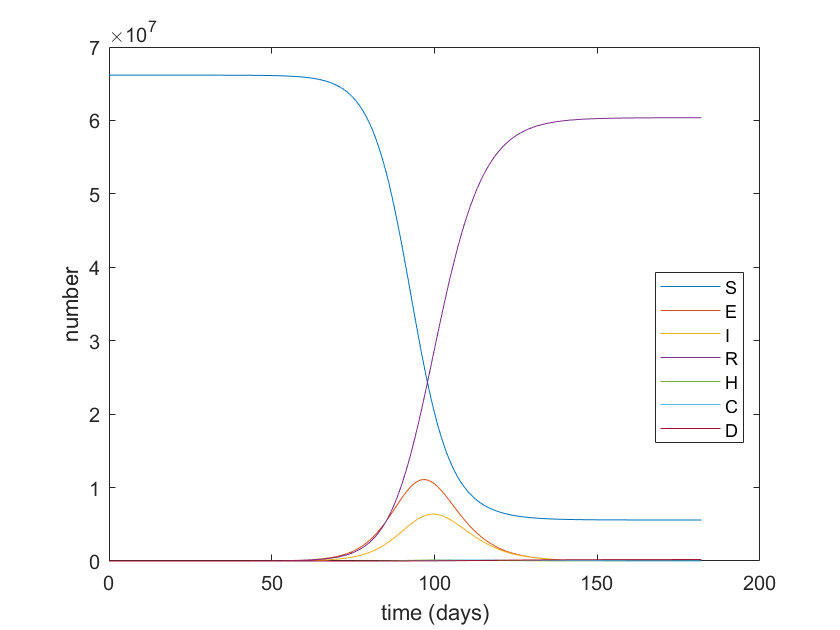
\includegraphics[width=0.45\textwidth]{neherlab-comparison/real-time-plot-1}~
    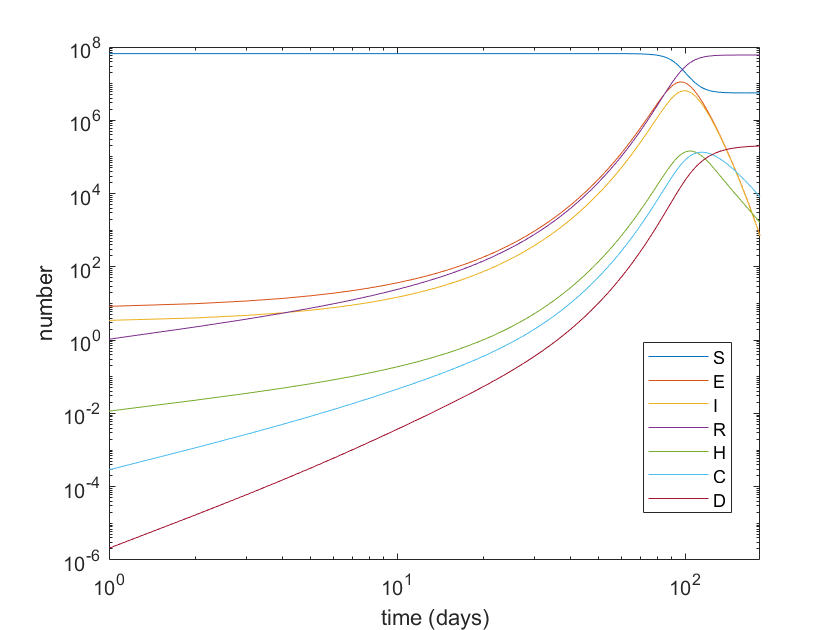
\includegraphics[width=0.45\textwidth]{neherlab-comparison/log-log-plot-1}
    \caption{Test run for Karnataka with a population $N = 66165886$ and initial exposed/infected population of 10, i.e. $E_4 = 7$, $I_4 = 3$ with no mitigation, no imports.}
    \label{fig:dynamics-no-mitigation}
\end{figure}

\begin{figure}[H]
    \centering
    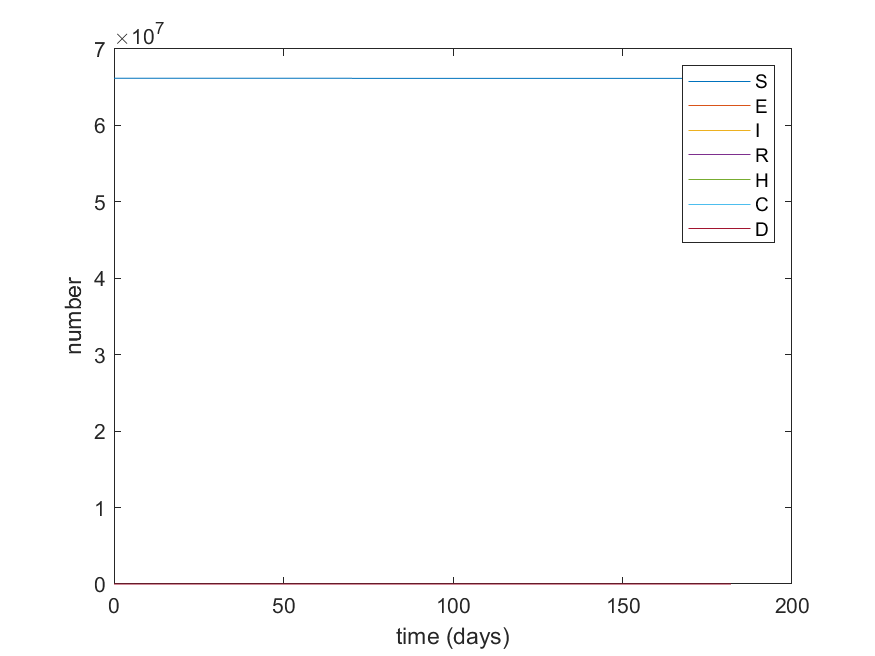
\includegraphics[width=0.45\textwidth]{neherlab-comparison/real-time-plot-2}~
    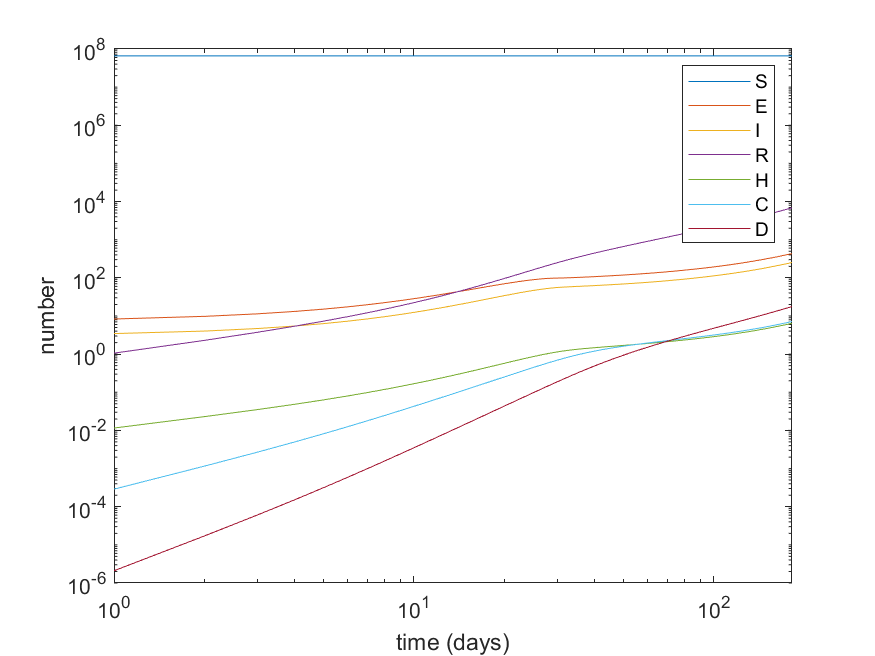
\includegraphics[width=0.45\textwidth]{neherlab-comparison/log-log-plot-2}
    \caption{Test run for Karnataka with a population $N = 66165886$ and initial exposed/infected population of 10, i.e. $E_4 = 7$, $I_4 = 3$ with strong mitigation, no imports}
    \label{fig:dynamics-strong-mitigation}
\end{figure}


\begin{figure}[H]
    \centering
    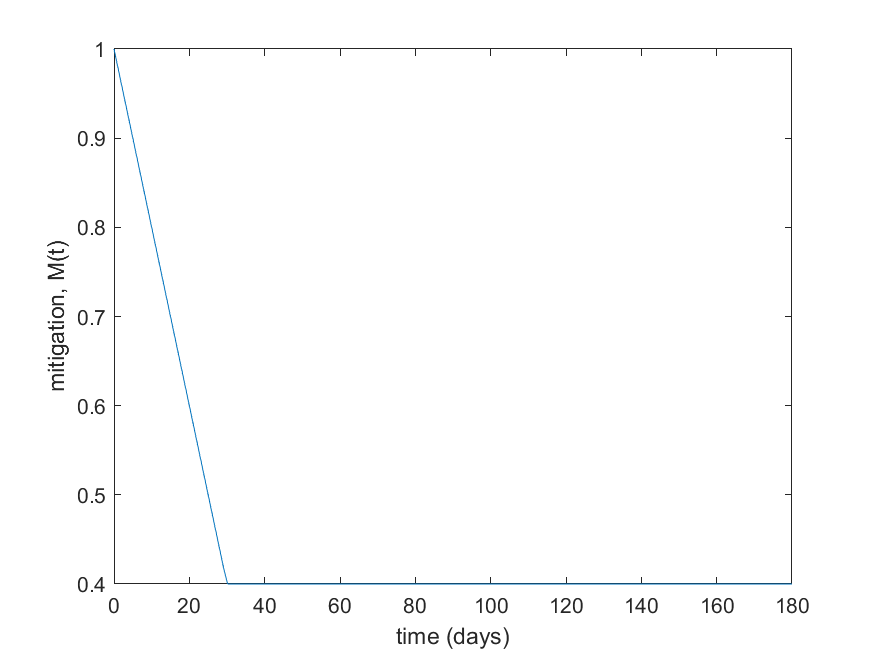
\includegraphics[width=\textwidth]{neherlab-comparison/strong-mitigation}
    \caption{Mitigation curve for Fig.\,\ref{fig:dynamics-strong-mitigation}}
\end{figure}


\section{Our model including economic demographic}

In our model we consider a city and several, $N_v$, villages. 
In each of them the population is divided into:
\begin{enumerate}
	\item 3 economic categories, into immobile poor, mobile poor and rich
	\item 3 age categories, into children (0-14), young (15-59) and old (60+) 
	\item 5 state, Susceptible (S), Exposed (E), Infectious (I), Recovered (R), Dead (D)
\end{enumerate}

While we will label the states with a capital letter as indicated next to the states in the list above, we will use a subscript to denote age (a) and economic (e) categories. Therefore, $S_{ae}, I_{ae},...$. The dynamics is given by the following reaction graph:

\begin{figure}[H]
	\centering
	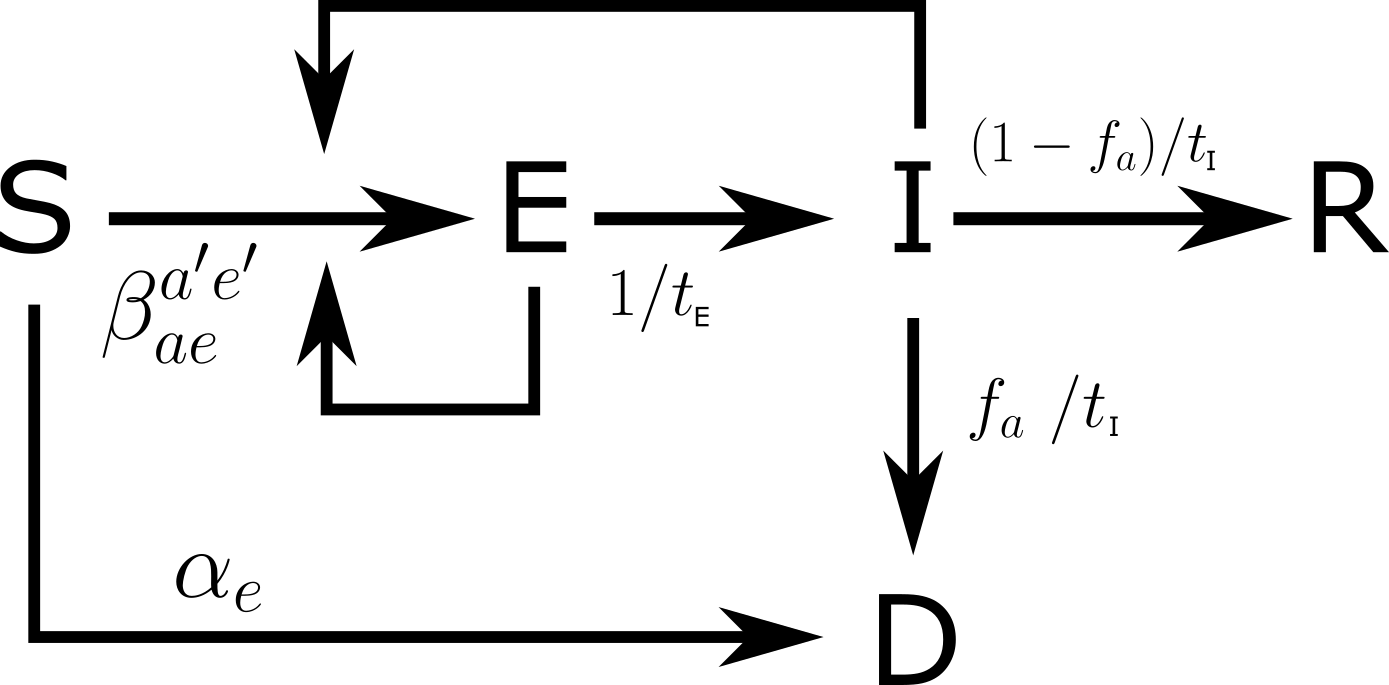
\includegraphics[width=\textwidth]{our_scheme}
\end{figure}

and the corresponding dynamics are given by the equations below

\begin{eqnarray}
\dbdt S_{ae} &=& - \sum_{a',e'} \beta^{ae}_{a'e'} S_{ae}(t) \bigg( I_{a'e'}(t) + E_{a'e'}(t) \bigg) + \mathcal{M}^{S}_{ae}(t)\\
\dbdt E_{ae} &=& \sum_{a',e'} \beta^{ae}_{a'e'}  S_{ae}(t) \bigg( I_{a'e'}(t) + E_{a'e'}(t) \bigg) - E_{ae}(t)/t_E + \mathcal{M}^{E}_{ae}(t)\\
\dbdt I_{ae} &=& E_{ae}(t)/t_E - I_{ae}(t)/t_I + \mathcal{M}^{I}_{ae}(t)\\     
\dbdt R_{ae} &=& (1- f_{a}) I_{ae}(t)/t_I  + \mathcal{M}^{R}_{ae}(t)\\
\dbdt D_{ae} &=& f_{a} I_{ae}(t)/t_I + \alpha_e S_{ae}(t)
\end{eqnarray}
Notice that the parameters have subscripts too. This shows that they dependent on the age (a) and economic (e) category too. The full list of these parameters and their meaning is provided below 

\begin{table}[H]
	\centering
	\begin{tabular}{l r} % c l}
		\toprule
		\textbf{Parameter} & \textbf{Symbol} \\ % & \textbf{Value} & \textbf{Units} \\
		\midrule
		interactions rate between $S_{ae}$ and $I_{a'e'}$ / $E_{a'e'}$  & $\beta^{ae}_{a'e'}$ \\ % & 2-3 & per day \\
%		reduction in interaction rate & $\zeta$ \\ %& 0-1 &  \\
%		mitigation & $M(t)$ & 0-1 &  \\
%		seasonal driving & $\varepsilon$ & 0 & \\
%		peak of seasonal effects & $t_{max}$ & Jan 2020 & time \\ 
		time spent in E (latency period) & $t_E$ \\ % & 5 & days \\
		time spent in I (infectious period) & $t_I$ \\ %& 3 & days \\
%		average hospitalisation time & $t_h$ & 4 & days \\
%		average time in ICU & $t_c$ & 14 & days \\
%		proportion of mild symptoms & $m_a$ & 0-1 & \\
%		proportion requiring critical care & $c_a$ & 0-1 & \\
		proportion for which the disease is fatal & $f_a$ \\ % & 0-1 & \\
		import rate & $\mathcal{M}$ \\
		\bottomrule
	\end{tabular}
	\caption{Parameters in our model}
	\label{table:our_model_parameters}
\end{table}











\begin{thebibliography}{20} 

\bibitem{NeherFeb2020} \url{https://neherlab.org/covid19/about}


\end{thebibliography}















\end{document}          